\chapter{Referencial Teórico}\label{chp:referencial}

Esse capítulo apresenta os principais conceitos desse trabalho. Entre esses conceitos destacam-se as definições do que são eventos, de fluxos de dados, de sistemas de processamento de eventos complexos e suas características principais, dos tipos de mudanças de conceito, do funcionamento do processo de aprendizado ou mineração em fluxos de dados. Além disso, inclui-se uma explicação detalhada sobre algoritmos de seleção de atributos e, finalmente, qual teste de hipótese será utilizado para validar os resultados deste trabalho.

\section{Fluxos de Dados}\label{sec:fluxos_dados}

Segundo o Glossário de Processamento de Eventos, desenvolvido e mantido pela \textit{Event Processing Technical Society} (ETS) 
\nomenclature{ETS}{\textit{Event Processing Technica Society}} 
\cite{Luckham2008}, um evento é qualquer acontecimento ou algo que está acontecendo. Por exemplo, uma transação financeira, o pouso de um avião, uma ocorrência natural como um terremoto, uma mudança de registros em um banco de dados, uma ocorrência cultural ou histórica, dentre outros. Um evento complexo é todo evento que represente um conjunto de outros eventos. Entretanto, esses acontecimentos são abstratos e precisam ser codificados em uma linguagem em que os computadores possam processá-los. Entende-se, portanto, que um evento em sistemas para processamento de eventos complexos (\textit{complex event processing systems} -- CEP)
\nomenclature{CEP}{\textit{Complex Event Processing}} 
é qualquer objeto que represente um determinado evento, e.~g. um registro de uma compra, um e-mail de confirmação de uma reserva de passagem aérea, uma mensagem enviada por um sensor elétrico, um documento de seguro médico dentre outros. Essas sequências de eventos, quando transformados em dados e transmitidos para os sistemas CEP, em alta velocidade e em grande volume, são denominados fluxos de dados. 

Um fluxo de dados $S = \{S_1, S_2, \ldots, S_n\}$ pode conter um ou mais eventos $S_i$, representados em tuplas. Cada tupla é composta por diferentes atributos, contendo informações relevantes ao evento que se refere. As características dos fluxos de dados são consideravelmente distintas daquelas encontradas em conjuntos de dados persistentes (\textit{offline}), segundo \citeonline{Ramirez-Gallego2017}. As principais diferenças são apresentadas na Tabela~\ref{tabela_diferencas}.

\begin{table}[!htb]
\centering
\caption[Principais diferenças entre fluxos de dados e dados persistentes]{Principais diferenças entre fluxos de dados e dados persistentes. Adaptadas de \citeonline{Ramirez-Gallego2017}}
\label{tabela_diferencas}
\begin{longtable}[c]{|p{7.5cm}|p{7.5cm}|}
\hline
\textbf{Fluxos de Dados} & \textbf{Dados Persistentes} \\ \hline
   Não são conhecidos previamente, mas disponibilizados sequencialmente  &             O conjunto de dados total é conhecido      \\ \hline
    Podem ser transmitidos em frequências completamente diferentes  &             Todas as tuplas estão presentes no conjunto inicial     \\ \hline
          São potencialmente infinitos  &             Os conjuntos são finitos     \\ \hline
                  Precisam ser analisados em um tempo limitado &            Os conjuntos podem ser acessados quantas vezes forem necessárias      \\ \hline
                  As características probabilísticas dos dados podem sofrer alterações ao longo do tempo &            Uma vez disponibilizados, os dados do conjunto não sofrem nenhum tipo de alteração      \\ \hline

\end{longtable}
\end{table}


Conforme indicado na Tabela ~\ref{tabela_diferencas},
as características dos fluxos não são conhecidas previamente. Os fluxos são
processados e analisados na medida em que chegam ao sistema, de modo sequencial, respeitando a ordem de chegada. Além disso, cada fluxo pode ser transmitido em uma frequência completamente diferente de outro. Embora alguns padrões possam ser encontrados, não é possível definir em que momento cada fluxo é transmitido. 

Como são potencialmente infinitos, à medida que começam a ser transmitidos, não se pode dizer quando o fluxo cessará. Por seu grande volume e alta velocidade, aliado à possibilidade de conterem informações críticas, esses fluxos precisam ser analisados em tempo limitado. Refazer o processamento e análise em fluxos já processados é, na maioria das vezes, inviável. 

Por fim, como principal fator que os diferencia dos dados persistentes, os fluxos de dados podem sofrer alterações em suas características probabilísticas ao longo do tempo
. Esse fenômeno é conhecido como Mudança de Conceito.

\section{Sistemas de Processamento de Eventos Complexos}\label{sec:complex_event}

De acordo com \citeonline{Gradvohl2016}, os sistemas CEP podem ser definidos como sistemas distribuídos de processamento de fluxos de dados, que recebem como entrada uma ou mais sequências de eventos (os fluxos de dados) e produzem uma saída, que também pode ser uma sequência de eventos. Visto que os fluxos de dados podem ser transmitidos por diferentes dispositivos ou aplicações, produzindo e transmitindo dados em tempo real, os sistemas CEP podem ser entendidos como sistemas de processamento \textit{online}. 


Os sistemas CEP são compostos por basicamente dois tipos de componentes: os componentes de \textit{software}, conhecidos como Operadores; e os componentes de \textit{hardware}, definidos como Nós de Processamento, onde os operadores são executados. Cada operador pode estar em apenas um nó de processamento, embora um mesmo nó possa armazenar e executar um ou mais operadores. Esses componentes são organizados para formarem um Grafo Acíclico Dirigido. Esse arranjo de operadores
é conhecido como a topologia de um sistema CEP. A Figura~\ref{fig:topologia} apresenta um exemplo de topologia em sistemas CEP.


\begin{figure}[!htb]
  \centering
    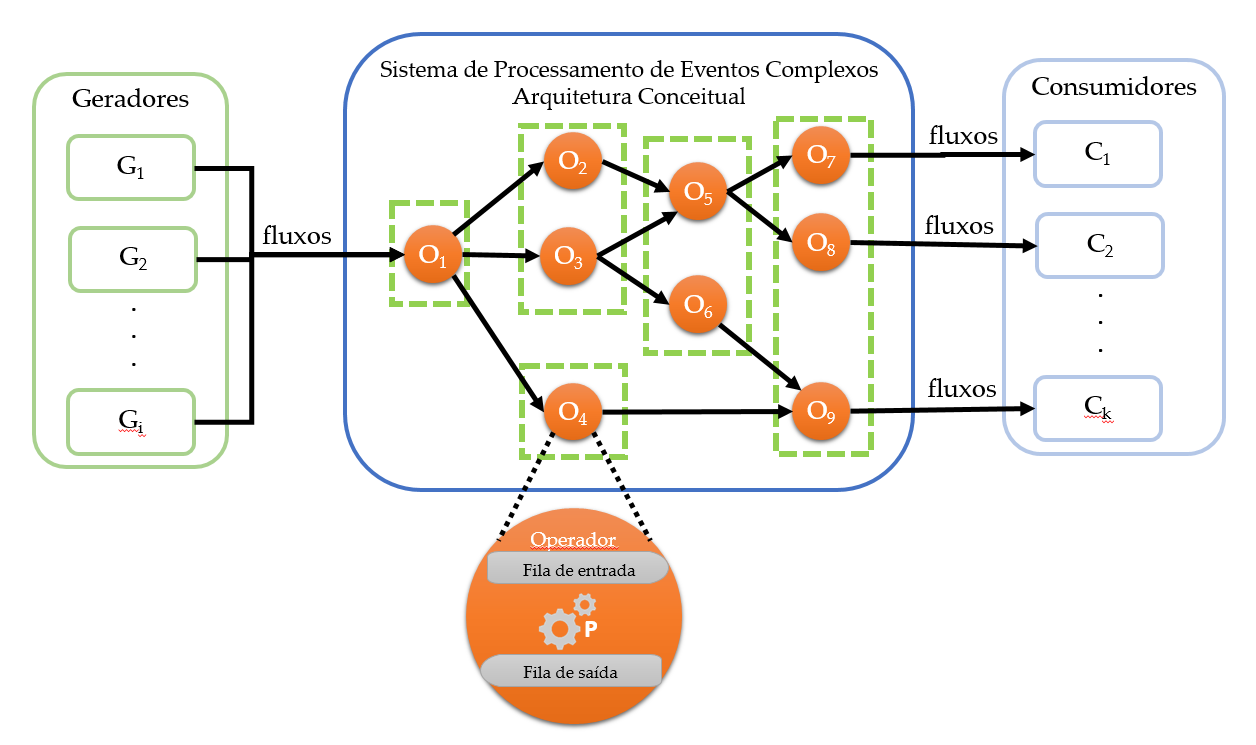
\includegraphics[width=.8\textwidth]{topologia.png}
    \caption{Representação de um sistema CEP, adaptado de \cite{Gradvohl2016}.}
    \label{fig:topologia}
\end{figure}

Conforme ilustra a Figura~\ref{fig:topologia}, dispositivos ou sistemas geradores de conteúdo enviam os dados, em formato de fluxos de dados, para processamento e análise dos sistemas CEP. Quando o fluxo é recebido pelo sistema CEP, suas tuplas são processadas e analisadas pelos operadores pertencentes à sua topologia que, após o processamento, reenviam as tuplas já processadas e analisadas para os demais operadores da topologia, até que todo o ciclo tenha sido finalizado. 

%[Andre] Adicionei uma quebra de parágrafo
Em cada operador, 
a tupla aguardará na fila de entrada até seu efetivo processamento. 
Após o processamento, o operador pode gerar uma nova tupla que será enviada para a fila de saída, 
até seu encaminhamento
para o próximo operador. Por fim, as tuplas são enviadas como fluxos de dados para os Sistemas Consumidores, que receberão os dados processados e analisados, prontos para serem consumidos. 

A etapa mais importante desse processo é o processamento das tuplas por parte dos operadores. Esse processamento pode ser tanto no sentido de analisar os dados recebidos, quanto de aplicar algum algoritmo em cima dos dados, para limpeza, redução ou filtragem, dentre
outras operações.

Em sistemas CEP, os usuários definem \textit{queries} ou regras que especificam como processar os eventos recebidos em formato de fluxos de dados. Conforme aponta \citeonline{Higashino2016}, embora hajam esforços para padronizar as \textit{queries} e garantir uma única linguagem para realização desse processamento, uma grande variedade de linguagens diferentes ainda é utilizada. \citeonline{Margara2011} classificam as linguagens existentes em três grupos distintos:

\begin{itemize}
\item \textbf{Declarativos}: os resultados esperados do processamento são declarados, ao invés de declarar qual fluxo de operadores o processamento deve seguir. Geralmente essas linguagens são derivadas de linguagens relacionais como a álgebra relacional e a SQL.

\item \textbf{Imperativos}: o usuário deve definir um plano para onde cada tupla deve ir e quais operadores deve processá-la. Cada operador transformará as tuplas recebidas em novas tuplas. No geral, os sistemas que trabalham com essa linguagem oferecem ferramentas visuais para definição das regras.

\item \textbf{Baseado em padrões}: linguagens utilizadas para detectar regras nas tuplas recebidas e quais ações devem ser tomadas quando as condições de atuação forem atingidas. Essas condições são definidas geralmente como padrões que são captados pela combinação do uso de operadores lógicos, relacionamentos e constantes de tempo. 
\end{itemize}


Conforme apontado por \citeonline{Higashino2016}, a base para o desenvolvimento dos sistemas CEP se deu à partir do estudo publicado por \citeonline{Luckham1997}.
Nesse estudo, o autor apresenta a ferramenta Rapide, um sistema de simulação para sistemas distribuídos. Por volta do mesmo período, a comunidade científica de banco de dados desenvolveu os primeiros sistemas para processamento de fluxos, como o Aurora \cite{Carney2003} e o STREAM \cite{Arasu2004}. Atualmente, existem diversos sistemas CEP em funcionamento, como o Apache Spark, Apache Storm, Apache Samza, MillWheel dentre outros \cite{Gradvohl2014}.


\section{Mineração em Fluxos de Dados}\label{sec:mineracao_fluxos} 

O método mais comum para extração de conhecimento de fluxos de dados é através do processo de classificação. Essa tarefa é conhecida por categorizar as instâncias de um fluxo de dados entre classes de acordo com suas relações ou afinidades. Assumindo um conjunto de possíveis classes $Y = \{y_1, \ldots, y_c\}$, um classificador constrói um modelo que prevê ou classifica as instâncias ainda não classificadas $\vec{x}_i$ para suas respectivas classes $y_i$.


O processo de classificação pode ser definido formalmente do seguinte modo: um conjunto de $n$ instâncias de treinamento na forma ($\vec{x}_i$, $y_i$) onde $y_i$ é um valor discreto que representa essa classe e $\vec{x}_i$ é um vetor que representa as tuplas, de tamanho $D$-dimensional, onde $D$ representa a quantidade de atributos que essa tupla contém.  Esses atributos podem conter valores categóricos, ordinais, numéricos ou uma representação das três formas. Um classificador é usado para produzir um modelo $f:\vec{x}_i \rightarrow Y$ que classificará as instâncias futuras \cite{Barddal2017}.

De acordo com a Teoria Bayesiana, a classificação pode ser colocada como uma função de probabilidades prévias de uma classe ($P \big[ y \big]$) e a função de densidade de probabilidade condicional ($P \big[ \vec{x} \vert y \big]$) para todas as possíveis classes $y_i \in Y$. A decisão de classificar uma instância em determinada classe é executada de acordo com a probabilidade posterior das classes, onde a Equação ~\ref{eq:bayes} define a probabilidade posterior de uma classe arbitrária $y_i$ e $P  \big[ \vec{x} \big] = \sum_{y_i\in Y} P  \big[ y_i \big] \times P  \big[ \vec{x} \vert y_i \big]$.

\begin{equation}
P  \big[ y_i \vert \vec{x} \big] = \frac{P  \big[ y_i \big] \times P  \big[ \vec{x} \vert y_i \big]}{P  \big[ \vec{x} \big]}	
\label{eq:bayes}
\end{equation}


Tratando-se de mineração em fluxos de dados, são três os principais desafios enfrentados: volume, velocidade e volatilidade. Volatilidade corresponde à um ambiente dinâmico em constante mudança. Volume e velocidade exigem que uma grande massa de dados sejam processado em um tempo limitado. 

%[Andre] Adicionei uma quebra de parágrafo
A princípio, iniciando a partir da primeira tupla recebida, a quantidade de dados aumenta constantemente de zero até potencialmente infinito. Isso exige que sejam utilizadas abordagens que possam se adaptar às mudanças, incorporando informações à medida em que se tornam disponíveis, processando de forma \textit{online} os casos que não possam ser armazenados. Deste modo, para que um algoritmo de mineração em fluxos de dados seja de fato eficiente, é preciso que o mesmo seja adaptável \cite{Krempl2014}.

Segundo 
\citeonline{Gama2010}, 
Algoritmos de Aprendizado Adaptáveis podem ser definidos formalmente do seguinte modo: seja $T_{t} = \{\vec{x}_{i},y_{y} : y = f(\vec{x}) \}$ um conjunto de exemplos disponíveis em um tempo $t \in \{1, 2, 3, \ldots, i\}$. Um algoritmo de aprendizado é adaptável se à partir da sequência de exemplos $\{\ldots, E_{j-1}, E_{j}, \ldots\}$ 
é produzida a sequência de Hipóteses $\{\ldots, H_{j-1}, H_{j}, \ldots\}$ onde cada hipótese $H$ só depende da hipótese anterior $H_{i-1}$ e do exemplo $E_i$. Neste sentido, um algoritmo de aprendizado adaptável requer duas operações: Incremento, quando um exemplo $E_k$ é incorporado no modelo de decisão; e Decremento, quando um exemplo $E_k$ é removido de um modelo de decisão.



\section{Mudanças de Conceito}\label{sec:concept_drift} 

Ao lidar com fluxos de dados, por suas características inerentes, entende-se que serão transmitidos em tempo real, formando um fluxo potencialmente infinito. São inúmeras as possibilidades de distribuição de dados, considerando esse cenário. Espera-se, portanto, que os dados evoluam ao longo do tempo, tornando o ambiente para análise e processamento de fluxos extremamente dinâmico. Essas mudanças ocorrem nos conceitos dos dados do conjunto. A Equação~\ref{eq: conceito} define um conceito C como um conjunto de probabilidades prévias das classes e funções de densidade probabilísticas das classes condicionais, segundo \citeonline{Nguyen2012}.

\begin{equation}
C =   \underset{y\in Y}{\bigcup} \big\{( P\big[ y_i \big],  P\big[ \vec{x} \vert  y_i \big]) \big\}
\label{eq: conceito}
\end{equation}

Portanto, seja $S$ um fluxo de dados com uma quantidade de tuplas $i_t$ com um conceito $C_t$. 
Para todo instante $t_i$ do fluxo, se $C_{t_i} = C_{t_i-1}$, então $C$ é um conceito estável. Caso contrário, se entre dois intervalos de tempo $t_i$ e $t_j = t_i + \Delta \ (\text{ com } \Delta \geq 1)  \ C_{t_i} \neq C_{t_j}$, então uma mudança de conceito aconteceu \cite{Barddal2017}.  
Sendo assim, as probabilidades prévias das classes  $P\big[ y_i \big]$ podem mudar, as probabilidades condicionais das classes $P\big[ \vec{x} \vert  y_i \big]$ podem mudar e as probabilidades posteriores de $P\big[ y_i \vert  \vec{x} \big]$ também podem variar. Essas características afetam a capacidade de classificação dos algoritmos de aprendizado \cite{Gama2014}.

Existem diversas formas em que uma mudança de conceito pode acontecer na distribuição probabilísticas dos dados ao longo do tempo. Desse modo, há várias maneiras de categorizar as mudanças que ocorrem em um conjunto de dados. Uma delas separa as mudanças de conceito por velocidade de mudança, enquanto a outra as divide pelo motivo da mudança \cite{Goncalves2014}. De acordo com \citeonline{Gama2014}, quanto à velocidade de mudança, as categorias são: súbita ou abrupta, incremental, gradual e recorrente. Já a respeito das razões de mudança, as mesmas podem ser reais ou virtuais. 

As razões de mudança são ilustradas na Figura~\ref{fig:razao_mudanca}. Uma mudança real ocorre quando há variações na relação $P\big[ y_i  \vert \vec{x} \big]$, ou seja, quando as tuplas de um fluxo de dados possuem uma legítima classe em determinado momento e outra legítima classe em outro momento. Em contrapartida, uma mudança virtual ocorre quando há mudanças apenas em  $P\big[ \vec{x} \big]$, quando a distribuição dos dados do conjunto (tuplas) é alterada, mas a relação entre os dados e o conceito (classe) permanece o mesmo. No geral, ambas ocorrem de forma conjunta \cite{Goncalves2014}.

\begin{figure}[!htb]
  \centering
    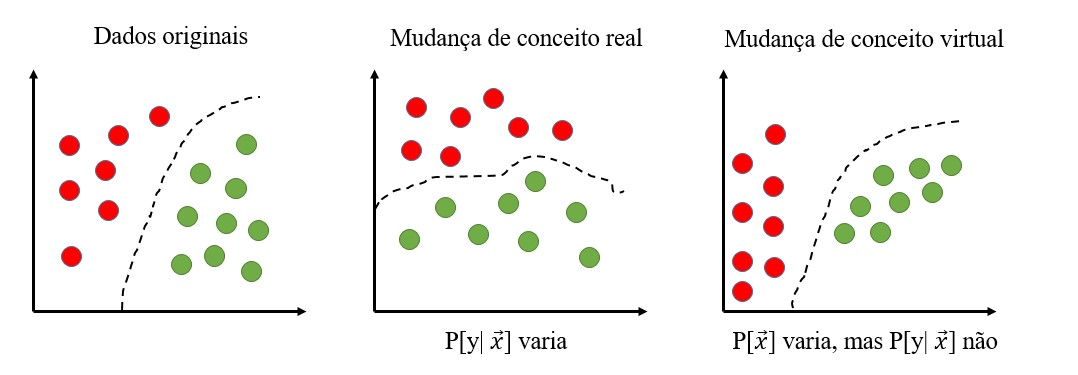
\includegraphics[width=.8\textwidth]{razao_mudanca.jpg}
    \caption[Tipos de mudanças de conceito, em relação à razão de mudança.] %[Andre] Entre colchetes está a legenda resumida. Entre chaves, a legenda completa.
    {Tipos de mudanças de conceito, em relação à razão de mudança. Círculos representam tuplas;  cores diferentes representam classes diferentes. Adaptado de \citeonline{Gama2014}.}
    \label{fig:razao_mudanca}
\end{figure}

O comportamento das mudanças em relação à velocidade de mudança é apresentado na Figura ~\ref{fig:tipos_conceito}. Nesta figura, é dado um exemplo de um conjunto de dados onde o conceito é referente a um atributo média. Conforme ilustrado, uma mudança de conceito súbita ou abrupta ocorre quando os fluxos variam de um conceito para outro repentinamente (e.~g. troca de um sensor por outro que possui uma calibragem diferente).

\begin{figure}[!htb]
  \centering
    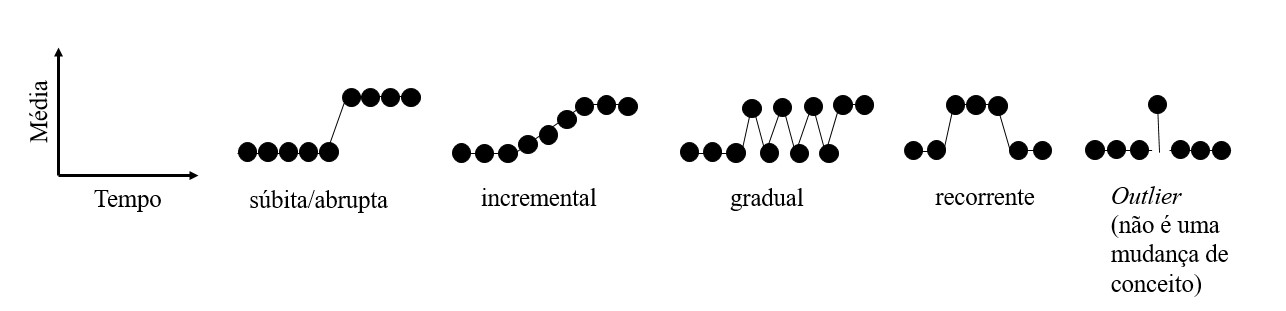
\includegraphics[width=.8\textwidth]{tipos_conceito.jpg}
    \caption[Tipos de mudanças de conceito, em relação à velocidade de mudança.]{Tipos de mudanças de conceito, em relação à velocidade de mudança. Adaptado de \citeonline{Gama2014}.}
    \label{fig:tipos_conceito}
\end{figure}

A mudança pode acontecer incrementalmente, consistindo em vários pontos intermediários dentre dois conceitos consideravelmente distintos (e.~g. um sensor que lentamente se torna menos preciso ao longo do tempo). Há, ainda, a mudança gradual, quando as mudanças não acontecem de forma abrupta, mas continuam voltando ao mesmo padrão antigo por um tempo (e.~g. tópicos de interesse em um jornal para uma pessoa que passará suas férias em outro lugar, onde o indivíduo não mudará repentinamente seus interesses, visualizando os interesses anteriores por um tempo). 

Finalmente, há a mudança recorrente, quando conceitos vistos previamente reaparecem após um intervalo de tempo (e.~g. vendas de um produto sobem no verão e caem no inverno). Por fim, é preciso distinguir a diferença entre mudanças de conceito e \textit{outliers}, que são pontos  que não representam corretamente a distribuição dos dados, podendo ser causados, por exemplo, por algum tipo de erro \cite{Han2006}.

\section{Seleção de Atributos}\label{sec:selecao_atributos} 

A alta dimensionalidade dos conjuntos de dados disponíveis atualmente, com o advento de \textit{Big Data}, representa um grande desafio para extração de conhecimento de grandes volumes de dados. Por exemplo, \citeonline{Weinberger2009} conduziram um estudo para filtragem colaborativa de \textit{spams} em plataformas de e-mail, lidando com conjuntos de dados que possuíam até 16 trilhões de atributos diferentes. \citeonline{Tan2014} fizeram um estudo similar, com conjuntos de dados reais e artificiais, contendo dezenas de milhões de instâncias com complexidade $O(10^{14})$ dada em função da quantidade de atributos. Essa grande quantidade de atributos é definida como ultra dimensionalidade.

A ultra dimensionalidade implica em uma necessidade massiva de memória e um alto custo computacional para treinamento e utilização dos algoritmos de aprendizado, além de dificultar a otimização de algoritmos pelo tamanho exaustivo de atributos, processo conhecido como ``Maldição da Dimensionalidade''. Esse termo, de acordo com \citeonline{Donoho2000}, foi apontado por Bellman em 1957 para descrever vários fenômenos que acontecem quando são analisados e organizados dados em grandes dimensionalidades, que não ocorrem se tratando de dados em baixa dimensionalidade. 

%[Andre] Adicionei uma quebra de parágrafo
Para lidar com 
a ``maldição de dimensionalidade''
, os conjuntos de dados podem ser sumarizados em representações menores porém mantendo, de certa forma, a qualidade original dos dados. Nesse caso, as representações menores possuem uma menor quantidade de atributos e uma menor quantidade de instâncias. Portanto, são utilizadas de forma mais eficiente e rápida do que suas versões originais. O processo para sumarização desses conjuntos de dados é conhecido como Redução de Dimensionalidade \cite{Bolon-Canedo2015}.

Uma das técnicas de redução de dimensionalidade é conhecida como Seleção de Atributos. Essa técnica visa detectar atributos relevantes e descartar atributos irrelevantes ou redundantes de um determinado conjunto de dados, obtendo uma representação reduzida do conjunto original, com perdas mínimas em termos estatísticos \cite{Han2006}. Existem diversas definições na literatura sobre a definição formal do que é a relevância de um atributo. Para este trabalho, serão utilizadas as definições propostas por \citeonline{Barddal2017}, descritas a seguir.

%Adição de uma descrição por extenso antes da definição formal

De acordo com a Definição~\ref{def:AtributoRelevante} 
a seguir
, assumindo um fluxos de dados $S_i$, que contém todos os atributos $D$ com exceção de um atributo $D_i$, entende-se que $D_i$ é relevante se e somente se, para toda tupla $S_i^{'}$, a não utilização do atributo $D_i$  reduzirá a capacidade geral de classificação de um algoritmo. Essa definição engloba duas possibilidades para um atributo ser estatisticamente significante para um processo de aprendizado: (i) está fortemente correlacionado com uma classe ou; (ii) em conjunto com outros atributos, forma um padrão fortemente correlacionado à uma classe.


\theoremstyle{definition}
\begin{definition}{\textbf{Atributo relevante}}\label{def:AtributoRelevante}
Assumindo $S_i = D\backslash \{D_i\}$, um atributo $D_i$ é \textbf{relevante} se e somente se

\begin{equation}
\exists S_i^{'} \subset S_i, \text{ sendo que } P\big[Y \vert D_i, S_i^{'}\big]\neq P\big[Y \vert S_i^{'}\big]
\end{equation}
De outra forma, $D_i$ é considerado \textbf{irrelevante}.
\end{definition}



Uma segunda definição é necessária para 
estabelecer
outro objetivo dos algoritmos de seleção de atributos, 
i.~e.
a remoção de atributos redundantes. Um atributo se torna redundante quando existem outros que produzem a mesma capacidade de classificação e aprendizado. Segundo a Definição~\ref{def:AtributoRedundante} 
a seguir
, assumindo um fluxos de dados $S_i$ que contém todos os atributos $D$, com exceção de um atributo $D_i$, entende-se que $D_i$ é redundante se e somente se, para toda tupla $S_i^{'}$, a capacidade de classificação de um algoritmo permanece a mesma, independente 
de
$D_i$ 
estar
ou não presente.

\begin{definition}{\textbf{Atributo redundante}}\label{def:AtributoRedundante}
Assumindo $S_i = D\backslash \{D_i\}$, um atributo $D_i$ é \textbf{redundante} se e somente se

\begin{equation}
\exists S_i^{'} \subset S_i, \text{ sendo que } P\big[Y \vert D_i, S_i\big] = P\big[Y \vert S_i\big] \wedge P\big[Y \vert S_i\big] \neq P\big[Y \vert S_i^{'}\big]
\end{equation}
\end{definition}


% \textbf{Definição 2.0} Assumindo $S_i = D\backslash \{D_i\}$, um atributo $D_i$ é \textbf{redundante} se e somente se

% \begin{equation}
% \exists S_i^{'} \subset S_i, \text{ sendo que } P\big[Y \vert D_i, S_i\big] = P\big[Y \vert S_i\big] \wedge P\big[Y \vert S_i\big] \neq P\big[Y \vert S_i^{'}\big]
% \end{equation}

Em relação à tarefa de seleção de atributos em fluxos de dados, 
esta
pode ser entendida como um problema de otimização, para obter o subconjunto ótimo $D^{*} \subseteq D$ de atributos que representam adequadamente os conceitos de determinados fluxos de dados. O principal objetivo dos algoritmos de seleção de atributos é remover atributos irrelevantes ou redundantes, enquanto mantém a distribuição probabilísticas das classes originais $P[Y]$. Para este trabalho, a definição formal da tarefa de seleção de atributos adotada será aquela proposta por \cite{Barddal2017}.

\begin{definition}{\textbf{Seleção de atributos}}\label{def:selecaoAtributos}
Assumindo o conjunto total de atributos $D$, o objetivo é selecionar um subconjunto de atributos $D^{*}$ que contém apenas informações relevantes de $S$. Suponha-se que a qualidade do subconjunto de atributos $D^{'} \subseteq D$ (argmax) é dada por $Q(.)$, então a tarefa de seleção de atributos pode ser definida conforme a Equação~\ref{eq:subconjuntoAtributos} a seguir, onde $d_{max}$ é o número de atributos selecionados.

\begin{equation}\label{eq:subconjuntoAtributos}
D^{*} = \text{argmax } Q(D^{'}) \text{ sujeito a } \vert D^{'} \leq \lceil d_{max}\rceil
\end{equation}
\end{definition}

%\textbf{Definição 3.0} Assumindo o conjunto total de atributos $D$, o objetivo é selecionar um subconjunto de atributos $D^{*}$ que contém apenas informações relevantes de $S$. Suponha-se que a qualidade do subconjunto de atributos $D^{'} \subseteq D$ (argmax) é dada por $Q(.)$, então a tarefa de seleção de atributos pode ser definida conforme a equação abaixo, onde $d_{max}$ é o número de atributos selecionados, arredondado para cima.

%\begin{equation}
%D^{*} = \text{argmax } Q(D^{'}) \text{ sujeito a } \vert D^{'} \leq d_{max}
%\end{equation}

Por fim, os algoritmos de seleção de atributos são divididos em três categorias distintas: filtros, envelopadores e métodos embarcados . As características e objetivos de cada um serão descritos a seguir, de acordo com as definições propostas por \citeonline{Guyon2003}.

\begin{itemize}
\item \textbf{Filtros}. Esses algoritmos aplicam medidas estatísticas para calcular uma pontuação para cada atributo. Os atributos são ranqueados baseados em suas pontuações e depois mantidos ou removidos. Esses métodos são, geralmente, univariados e consideram que cada atributo é independente de outro. Os algoritmos de filtragem são independentes do processo de classificação e aprendizado e possuem um baixo custo computacional. 
\item \textbf{Envelopadores}. Esses algoritmos consideram a seleção de atributos como um problema de busca. Envelopadores utilizam um classificador para avaliar a acurácia de cada combinação de atributos, até que a melhor combinação seja atingida. Como vantagem, esses métodos possuem um bom desempenho em fluxos de dados com mudanças de conceito, conforme aponta \citeonline{Ramirez-Gallego2017}, visto que sempre que novos fluxos são recebidos, o processo de aprendizado é refeito. Entretanto, uma desvantagem desses métodos é o alto custo computacional, vista a quantidade de operações necessárias para se atingir o resultado.
\item \textbf{Embarcados}. Os algoritmos embarcados selecionam os atributos durante o processo de treinamento de um classificador, sendo geralmente utilizados para determinados tipos de algoritmos. Conforme ilustra \citeonline{Barddal2017}, o aprendizado por árvores de decisão pode ser considerado um método embarcado, visto que a construção da árvore e a seleção de atributos estão interligadas, embora o processo de seleção de atributos em si seja através de filtragem.
\end{itemize}

\section{Teste de Hipótese}\label{sec:testeHipotese}

Com o objetivo de avaliar estatisticamente os resultados obtidos com os experimentos, um teste de hipótese foi utilizado. Esse tipo de teste garante  que os resultados não foram obtidos ou gerados aleatoriamente e seguem uma distribuição lógica. Neste trabalho, o teste não-paramétrico de Friedman \cite{Demsar2006} foi selecionado, por ser o mais indicado quando a quantidade de algoritmos avaliados é maior que 2.

O teste não-paramétrico de Friedman utiliza um sistema de \textit{ranking}, onde o melhor algoritmo obtém o \textit{rank} 1, o segundo melhor o \textit{rank} 2 e assim por diante. Seja $r^{j}_i$ o \textit{rank} do resultado do $j$-ésimo elemento de $k$ algoritmos utilizando o $i$-ésimo elemento de $N$ conjuntos de dados. O teste de Friedman compara os $rankings$ médios dos algoritmos, $R_j = \frac{1}{N} \sum_{i} r^{j}_i$. Considerando a hipótese nula, que afirma que todos os algoritmos são equivalentes e, portanto, seus \textit{ranks} R devem ser iguais, a Equação~\ref{eq:Friedman} apresenta a fórmula, considerando $k - 1$ graus de liberdade. Para esse teste, é necessário a definição de um intervalo de confiança, dado pela variável $\alpha$. Neste trabalho, $\alpha$ é definida com o valor $0,05$.

\begin{equation}\label{eq:Friedman}
\chi^{2}_{F} = \frac{12N}{k(k+1)} \Big[  \sum_{\substack{j}} R^{2}_{j} - \frac{k(k+1)^{2}}{4}\Big]
\end{equation}

Caso a hipótese nula seja rejeitada, isso indica que os algoritmos não são equivalentes. Desse modo, uma segunda validação pode ser efetuada, conhecida como teste \textit{post-hoc}. Esse teste busca avaliar estatisticamente se um determinado algoritmo possui, de fato, resultados superiores ou inferiores aos demais. Essa comparação pode ser feita considerando $n \times n $ comparações, quando vários algoritmos são comparados entre em si em busca de validação de qual possui o melhor resultado dentre todos,  ou $1 \times N$ comparações, quando os resultados dos algoritmos são comparados aos resultados de um algoritmo de controle. Por exemplo, em situações onde um novo algoritmo é desenvolvido e deve ser comparado à outro já existente na literatura.

Neste trabalho, consideramos $ 1 \times N $ comparações, visto que o objetivo principal é verificar se os algoritmos de seleção de atributos possuem um desempenho superior ou inferior à classificação sem utilização de métodos de redução de dados, considerando apenas a versão incremental do NB. Este último é configurado como controle.

Para execução do teste \textit{post-hoc}, utilizando os \textit{ranks} trabalhados anteriormente no teste de Friedman, algumas opções diferentes de testes podem ser selecionadas. Para este trabalho, foi definida a utilização do teste de Bonferroni-Dunn \cite{Demsar2006}. Esse teste fornece um valor de diferença crítica baseado no valor de $\alpha$ e na quantidade de algoritmos avaliados. O desempenho de dois ou mais algoritmos é considerada significantemente diferente se a diferença entre seus \textit{rankings} médios for maior ou igual a diferença crítica. Caso a diferença seja menor que a diferença crítica, considera-se que os desempenhos dos algoritmos são estatisticamente equivalentes. A Tabela~\ref{tab:bonferroni} apresenta algumas diferenças críticas para esse teste, considerando $\alpha = 0,05$.


\begin{table}[!ht]
\centering
\caption[Diferenças críticas para o teste de Bonferroni-Dunn.]{Diferenças críticas para o teste de Bonferroni-Dunn por quantidade de algoritmos, considerando $\alpha = 0,05$. A quantidade de algoritmos deve incluir o algoritmo de controle. Adaptado de \citeonline{Demsar2006}}
\label{tab:bonferroni}
%[Andre] Deixei todas as colunas centralizadas, exceto a primeira.
\begin{tabular}{cccccccccc}
\hline
$\alpha $& 2 & 3 & 4 & 5 & 6 & 7 & 8 & 9 & 10\\ \hline
0,05 & 1,960 & 2,241 & 2,394 &  2,498 &  2,576 &  2,638 &  2,690 &  2,724  & 2,773 \\ \hline
\end{tabular}
\end{table}

\section{Considerações finais deste capítulo}

Este capítulo apresentou os conceitos e características principais dos fluxos de dados, o que são sistemas de processamento de eventos complexos, os tipos de mudança de conceito que podem ocorrer na distribuição probabilísticas dos fluxos. Além disso, neste capítulo explicou-se o que são algoritmos de seleção de atributos, bem como definiu-se o que são atributos relevantes, irrelevantes e redundantes. Por fim, foi apresentado um método de teste de hipótese e teste \textit{post-hoc} para validação estatística dos resultados. Esses conceitos são importantes para se implementar os algoritmos de seleção de atributos como um método de redução em fluxos de dados.

